\documentclass[12pt, a4paper]{scrartcl}
\usepackage[utf8]{inputenc}
\usepackage{graphicx}
\usepackage{amsmath, amsthm, amssymb, textcomp}
\usepackage{setspace}
\usepackage{paralist}
\usepackage{graphicx}
\usepackage{caption}
\graphicspath{{WSK_im/}} %Graphic is in a folder named WSK_im in the currend directory
\usepackage{float}
\usepackage{authblk}
\renewcommand\Authfont{\fontsize{12}{14.4}\selectfont}
\title{Bayesian probability theory - Lesson 7:\\
Parameter and model estimation and classification}

\author{Wolfgang von der Linden, Gerhard Dorn, Johanna Moser}
\date{Transcript}

\begin{document}
\setlength{\parindent}{0pt}
\maketitle
\onehalfspacing

Welcome to unit 7 of the course on Bayesian probability theory. My
name is Wolfgang von der Linden and I will enable you to help Captain
Bayes and her crew to fit data by \textbf{model functions} and to learn the basics of
\textbf{parameter estimation, prediction} and \textbf{classification}
of data as well as on \textbf{model selection}.
\begin{itemize}\item We will learn how to apply Bayes theorem to \textit{derive} the probability
distribution for the parameters of an assumed model,
\item We will learn how to apply this probability distribution in the \textit{interpolation} 
of data to help Captain Venn find his treasure
\item We will learn how to \textit{classify} sea areas to be a nature reserve for
frogfish or a general fishing ground.
\end{itemize}


We begin with the classical \textbf{regression problem}. It is described as follows:\\
Let there be a \textit{set of measured data $d_{\nu}$} that depend on some \textbf{pivot points $x_{\nu}$}%7_1
\begin{figure}[H]
	\centering
	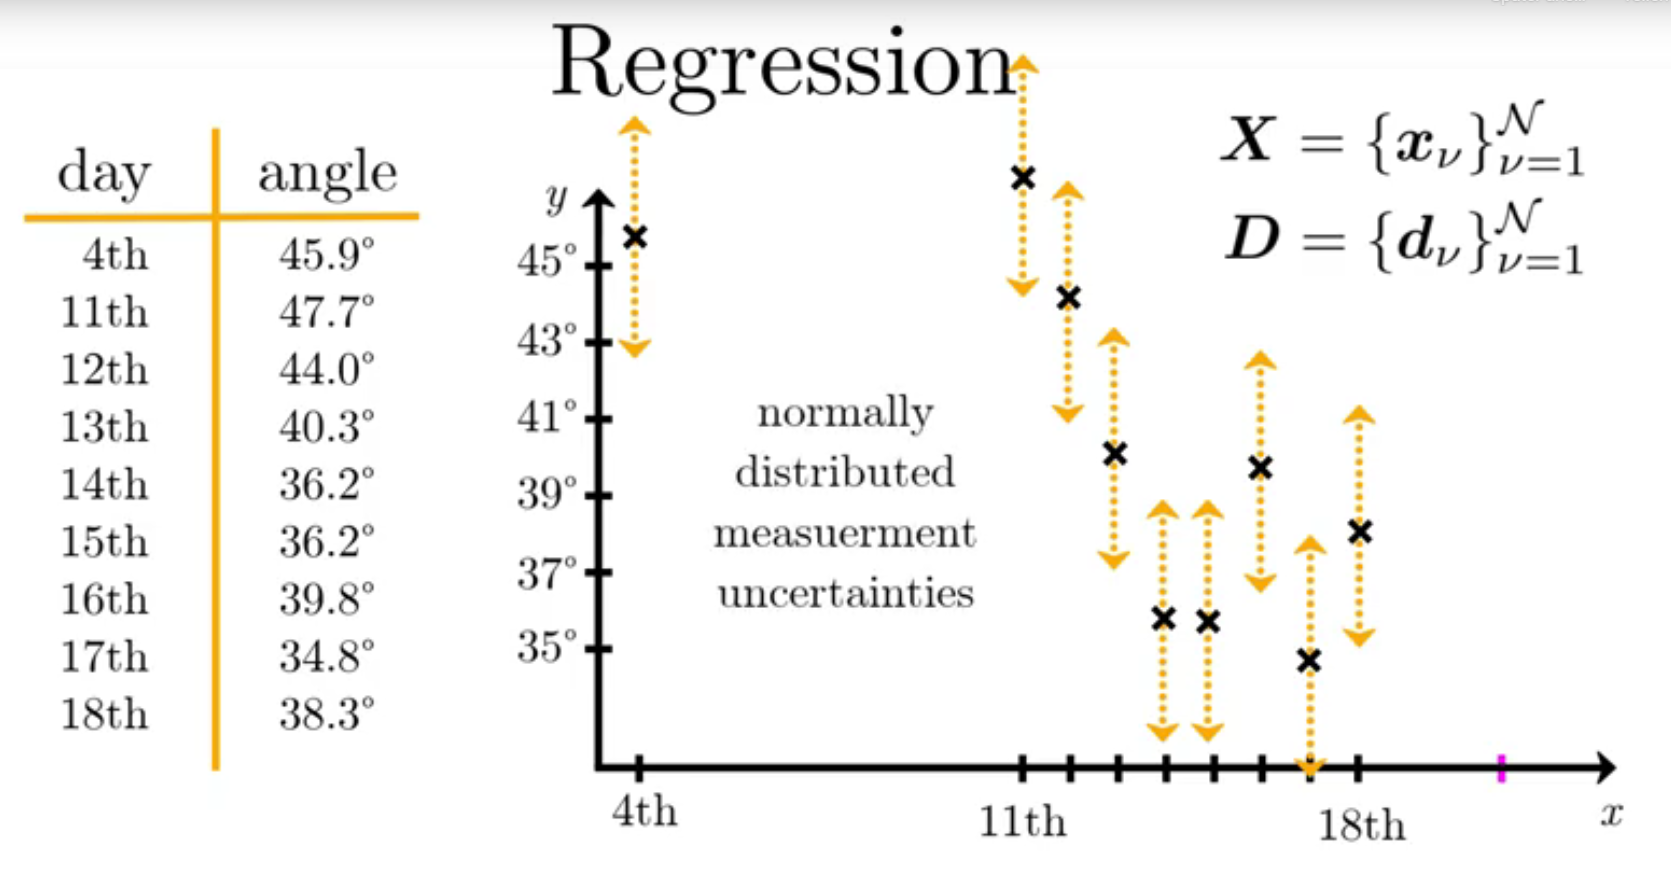
\includegraphics[width=0.75\textwidth]{7_1.png}
\end{figure}
These data points can be represented in an $x$-$y$ diagram. 
The measurements are in general not exact but have some uncertainty that obey a certain distribution.
In most cases like in the situation of Captain Venn these
are additive \textbf{Gaussian uncertainties}.
Next we assume that without the experimental uncertainty there is a \textit{relation}
between intrinsic data and the pivot points that can be described by a
\textit{deterministic} function, for instance a physical law that depends on some parameters.\\
\[y_{\nu} = f(x_{\nu},\vec{a})\]

\textit{Then the measured data can be described by adding the measurement uncertainty to the deterministic 
model function.}\[d_{\nu}=f(x_{\nu},\vec{a})+\eta_{\nu}\]


Now the goals of regression are twofold:\\

Firstly \textbf{Parameter estimation}: We would like to investigate the relation between 
measurement values $d_{\nu}$ and pivot points $x_{\nu}$ and therefore \textit{determine
the model and its parameters $\vec{a}$, their uncertainty $\sigma_{\vec{a}}$ and covariance $\text{CoV}(a_i,a_j)$}. 
In the case of Captain Venn and his starpath problem the goal is to find 
the laws of how the stars or rather the earth move. The model could
include the rotation of the earth around a tilted axis with respect to
the elliptic orbit around the sun. The parameters could represent the
duration of such a rotation and the orbital period.\\

The second aim of regression is to \textbf{predict the values $y^*$} of the function at
additional pivot points $x^*$ and their corresponding uncertainty. These
additional pivot points could be such, that it was not possible to realize
a measurement at these points. (Remember the case of Captain Venn
who was not able to determine the angles of the star Arcturus in the
shortest night of the year due to bad weather.)\\

Another important application is to \textbf{extrapolate} physical properties from a small scale
experiment to a larger one as is for instance done in fusion plasma reactors.\\

\section*{Parameter estimation}
Now we come to parameter estimation.
For your orientation we recapitulate the \textit{classical regression procedure} before
we introduce the probabilistic approach.
As described before we assume we have a suitable model $y_{\nu}=f(x_{\nu},\vec{a})$, which is for instance given by physical 
laws or is obvious due to a visible trend of the data. 
A very prominent choice are \textbf{linear models} in which
one uses a linear combination of suitable ansatz functions $\phi_i (x)$ with
the coefficients being the parameters. 
\[f(x,\vec{a})=\sum_i \phi_i(x)a_i\]

Based on the model function, a \textbf{cost function $\chi^2_{\vec{a}}$} is introduced that \textit{quantifies deviation between 
model function and data}. A very common cost
function is the \textbf{root mean square function}.\\
\begin{equation*}\boxed{\chi^2_{\vec{a}}=\sum_{\nu=1}^N\frac{d_{\nu}-f(x_{\nu},\vec{a})^2}{\sigma_{\nu}^2}
}\end{equation*}\\
 Sometimes the individual contributions get a weight $\sigma_{\nu}^2$
according to the reliability of the measured data.
Outliers thus have a very strong impact on the cost function.\\

In the next step the cost function is \textit{minimized} with respect to the model parameters. This 
is the so-called \textbf{least squares approach}. In the case of linear regression in combination 
with a quadratic cost function the
minimization leads to a matrix equation where the columns of the matrix $M$ are given by the ansatz
functions evaluated at the pivot points.\\%7_2
\begin{figure}[H]
	\centering
	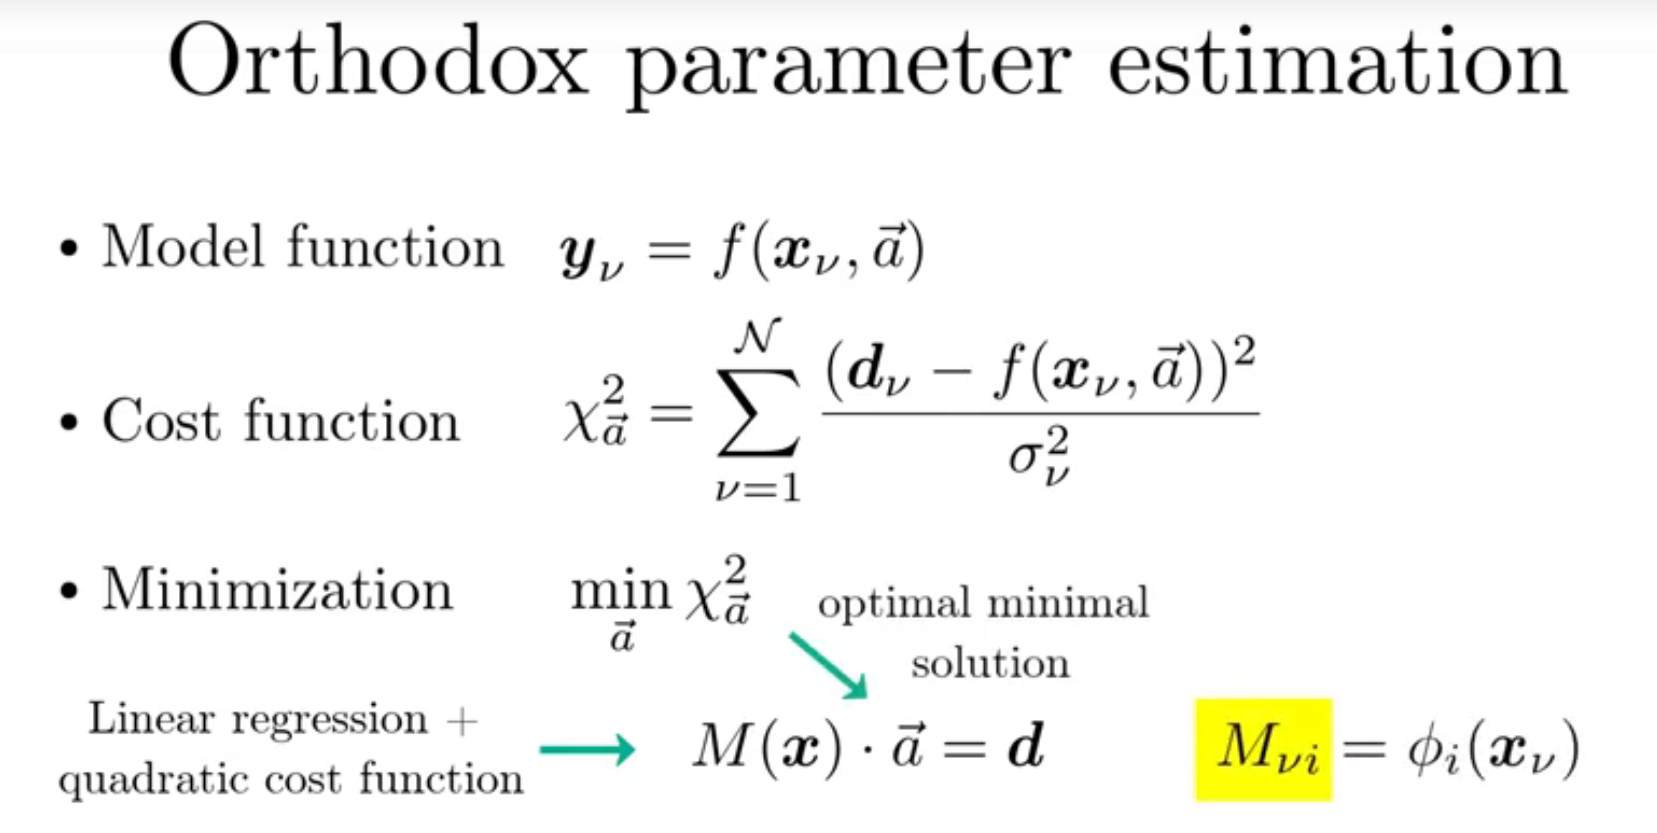
\includegraphics[width=0.75\textwidth]{7_2.png}
\end{figure}

If one is not entirely sure about the model function in a final step, one can evaluate the model function and
discuss whether is has a reasonable behaviour. 
This would lead to the field of \textbf{hypothesis testing}.\\


Now we come to \textbf{Bayesian parameter estimation}.
We have already mentioned several times that probability theory represents the consistent
calculus for dealing with uncertainty. The general approach is the following:\\

First we have to \textit{fix all assumptions} like ``the measurement are given for certain pivot points'',
``the data can be described by an assumed model'', ``the experimental noise follows a given distribution'' 
and so on. Then we have to \textit{specify the questions} we are interested in, like: ``What 
are the values of the parameters?'' ``What would be the value of the measured quantity at a new pivot point?''
``Is the assumed model the right one?'' ``What if there are \textbf{outliers}, which means there are individual data points that are \textit{corrupted
by external influences and do not obey the assumed error statistics}?''\\

Finally, we compute the corresponding probabilities. 
We will see at the end of this section when and under which conditions the previously presented statistical procedure is justified. \\

\section*{Probability density of the parameters}
The \textbf{probability density of the parameters} $\vec{a}$ in the light of the measured data $\boldsymbol{D}$ is the \textbf{posterior probability} that can
be simplified by Bayes theorem.
\begin{equation*}\boxed{p(\vec{a}|\boldsymbol{D},X)=\frac 1Z p(\boldsymbol{D}|\vec{a},X)p(\vec{a})
}\end{equation*}\\
 The normalization $Z$ is independent of the parameters and can be determined in the end.
The prior probability $p(\vec{a})$ encodes our \textit{knowledge about the parameters before we take into account the experimental data}.
If nothing is known at all, the most ignorant prior is the \textbf{uniform prior}; maybe within
certain parameter ranges. We will discuss in the next unit how ignorant
priors can be determined purely based on considerations of symmetries and
invariances.\\
A crucial element in Bayes theorem is the \textbf{likelihood} $p(\boldsymbol{D}|\vec{a},X)$.
If the measurement errors are uncorrelated the likelihood factorizes.
\[ p(\boldsymbol{D}|\vec{a},X)=\prod_{\nu} p(\boldsymbol{d}_{\nu}|\vec{a},x_{\nu})\]
In the case of additive Gaussian noise with noise level $\sigma_v$ we can express the
likelihood of one data point given by the model function $f$ and the parameters $\vec{a}$.%7_3
\begin{figure}[H]
	\centering
	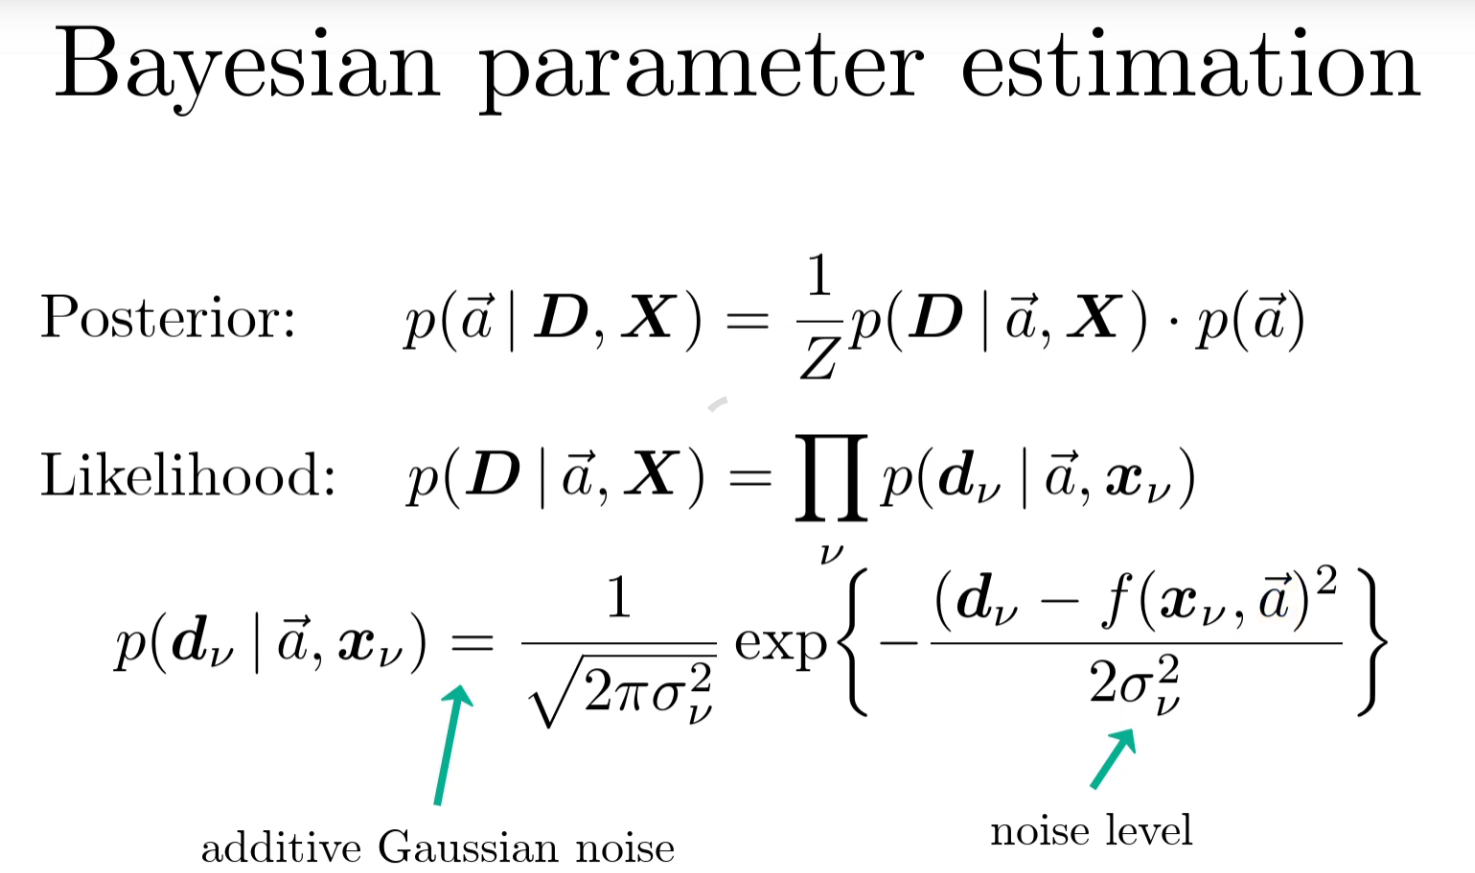
\includegraphics[width=0.75\textwidth]{7_3.png}
\end{figure}
Since we are interested in the probability density of the parameters $\vec{a}$,%%
we only need the terms that depend on them. We can replace the product
of the exponential by the exponential of the sum.
\begin{equation*}\boxed{ p(\boldsymbol{D}|\vec{a},X)\propto \exp\left[-\sum_{\nu}\frac{\boldsymbol{d}_{\nu}-f(x_{\nu},\vec{a})^2}{2\sigma_{\nu}^2}\right]=\exp\left[-\frac 12 \chi_{\vec{a}}^2\right]}\end{equation*}\\

This misfit term $\chi_{\vec{a}}^2$ corresponds to the \textbf{least squares cost function} which we
saw in the classical regression procedure. 
If there are uncertainties $\sigma_{x,\nu}, \sigma_{y,\nu}$ in both coordinates and if the regression
function is linear in $x$ $f(x,\vec{a})=a_1x+a_2$ then the misfit is given by the following expression:
\[\chi_{\vec{a}}^2=\sum_{\nu}\frac{(\boldsymbol{d}_{\nu}-a_2-a_1x_{\nu})^2}{\sigma_{y,\nu}^2+a_1^2\sigma_{x,\nu}^2}\]

In summary we find the following probability density function for the parameters:
%7_4
\begin{figure}[H]
	\centering
	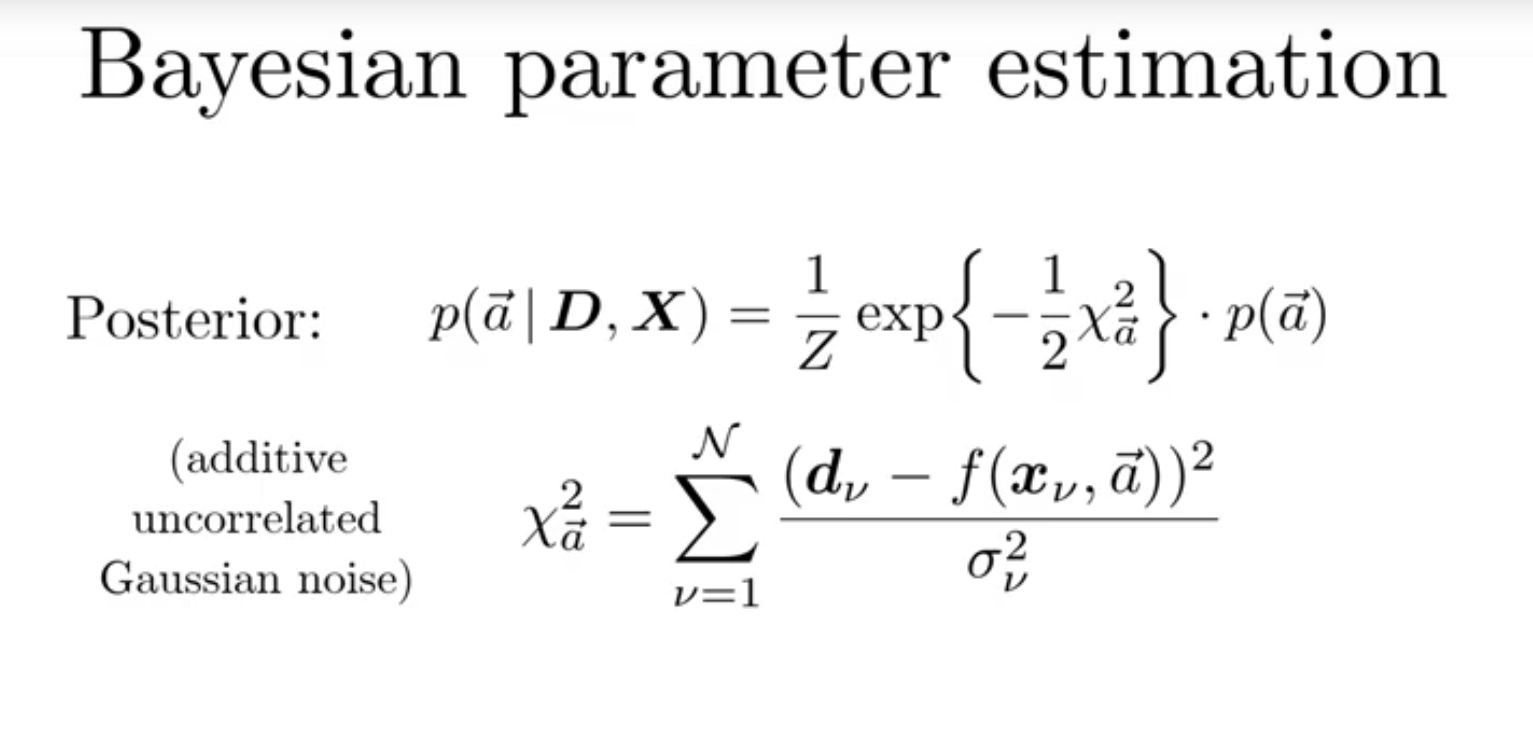
\includegraphics[width=0.75\textwidth]{7_4.png}
\end{figure}
More on the difference between pdfs and probability distributions will follow in the next unit.\\

An obvious way to decide on the parameters is to take the \textit{maximum of the posterior probability density} - the so-
called \textbf{MAP solution}. In the case of a flat prior this solution is
equal to the maximum likelihood. The\textbf{ Maximum Likelihood (ML)} choice of
the parameters is the basis of parameter estimation in conventional statistics.
If in addition the likelihood is \textit{Gaussian}, as in the present case, then the
MAP and ML solution is obtained by \textit{minimizing} $\chi_{\vec{a}}^2$, which is the
\textbf{Least-Squares} method that we discussed before.\\%7_5
\begin{figure}[H]
	\centering
	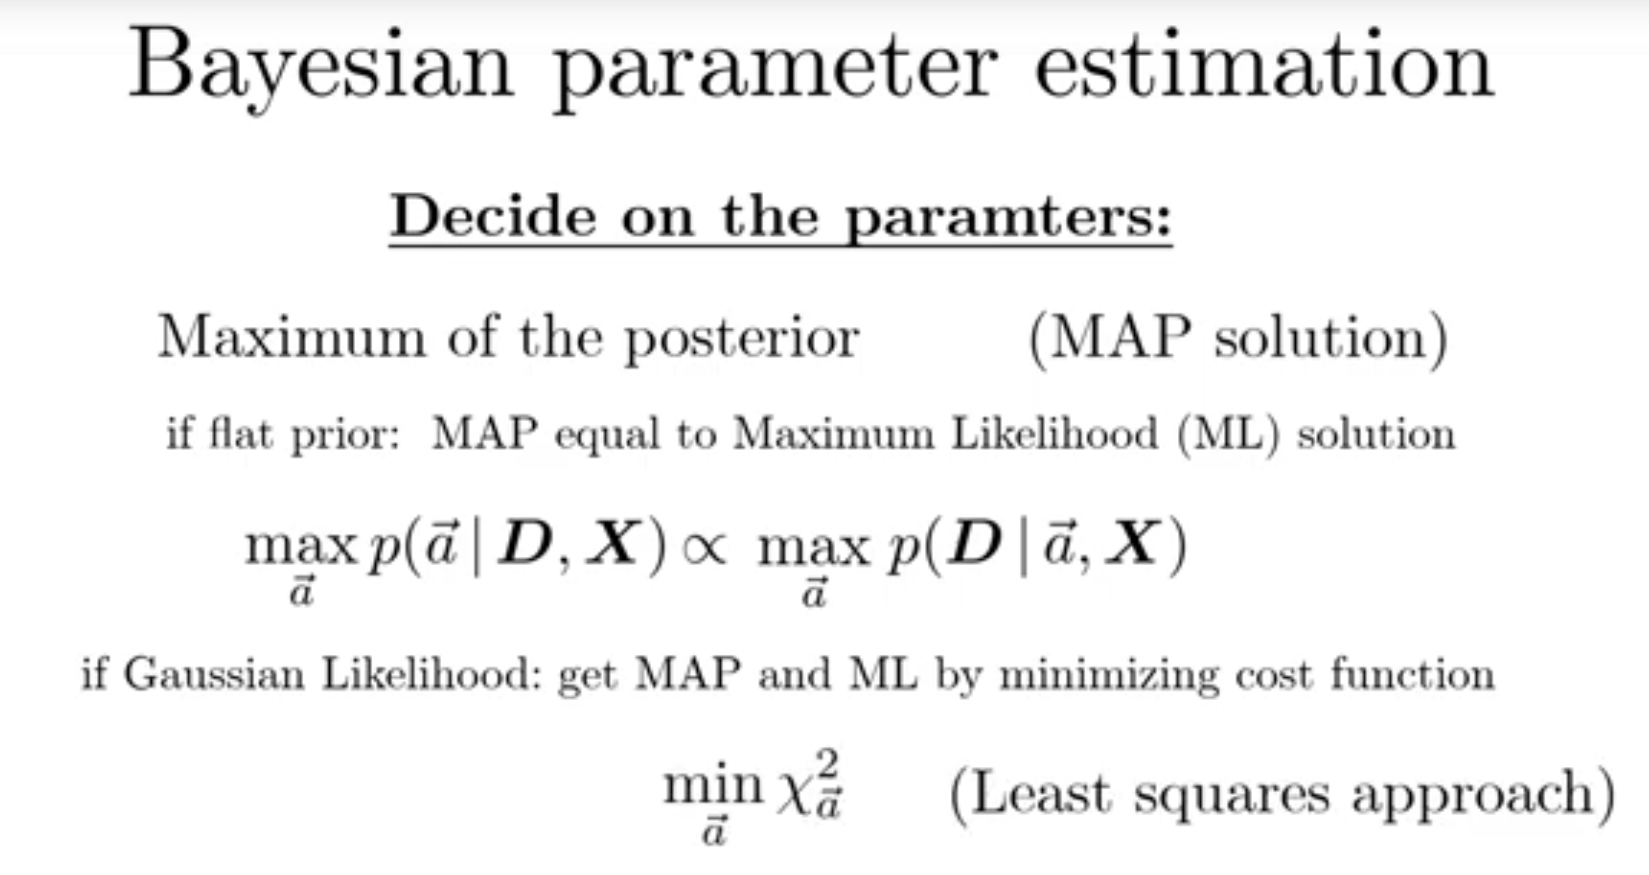
\includegraphics[width=0.75\textwidth]{7_5.png}
\end{figure}
\textit{This shows that the least squares approach is \textit{only applicable} in the case of Gaussian 
experimental noise and if we have no (or if we ignore) prior knowledge about the parameters.} \\

In general the MAP and hence ML solution is not very robust and highly
susceptible to noise. In particular if the likelihood is not \textbf{unimodal}, which means it has \textit{several peaks}, 
the maximum can be misleading if it does not carry the \textit{dominant probability mass}.
A more reliable characterization of the parameters is given by the \textbf{posterior
mean}.
Here we finally need the normalization, which can be obtained by the following integral.%7_6
\begin{figure}[H]
	\centering
	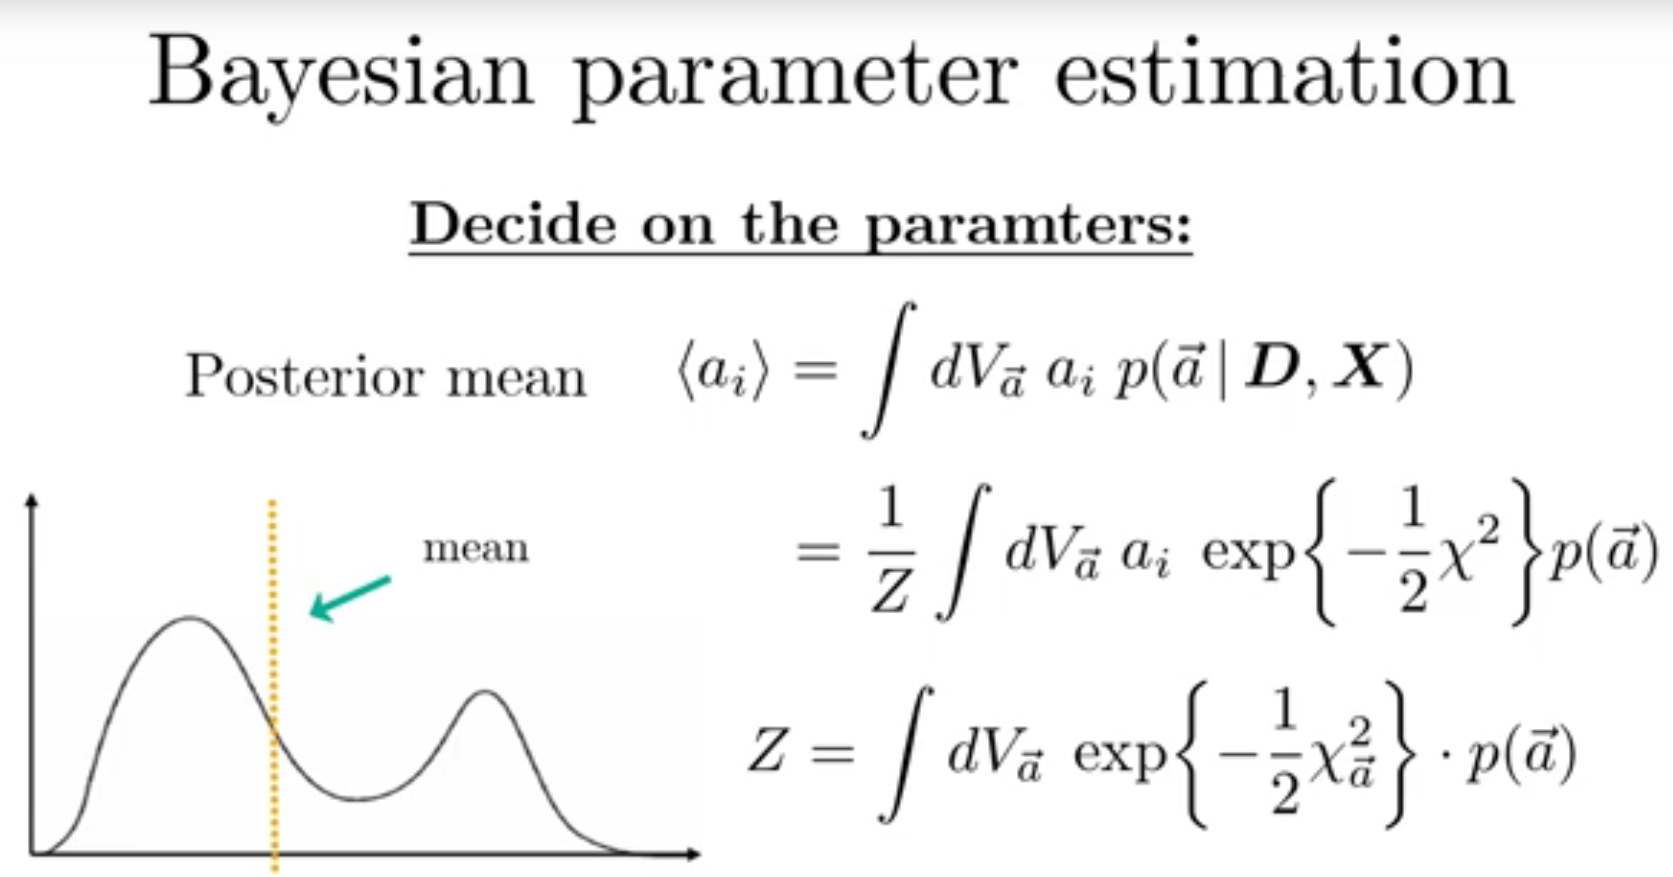
\includegraphics[width=0.75\textwidth]{7_6.png}
\end{figure}

It cannot be overstressed that a single value for the parameters, be it given
by the MAP or the mean, is \textit{meaningless, if we do not know the \textbf{uncertainty}}.
The uncertainty can be quantified by the \textbf{variance}.
In many cases also the \textbf{covariance} is of great interest.%7_7
\begin{figure}[H]
	\centering
	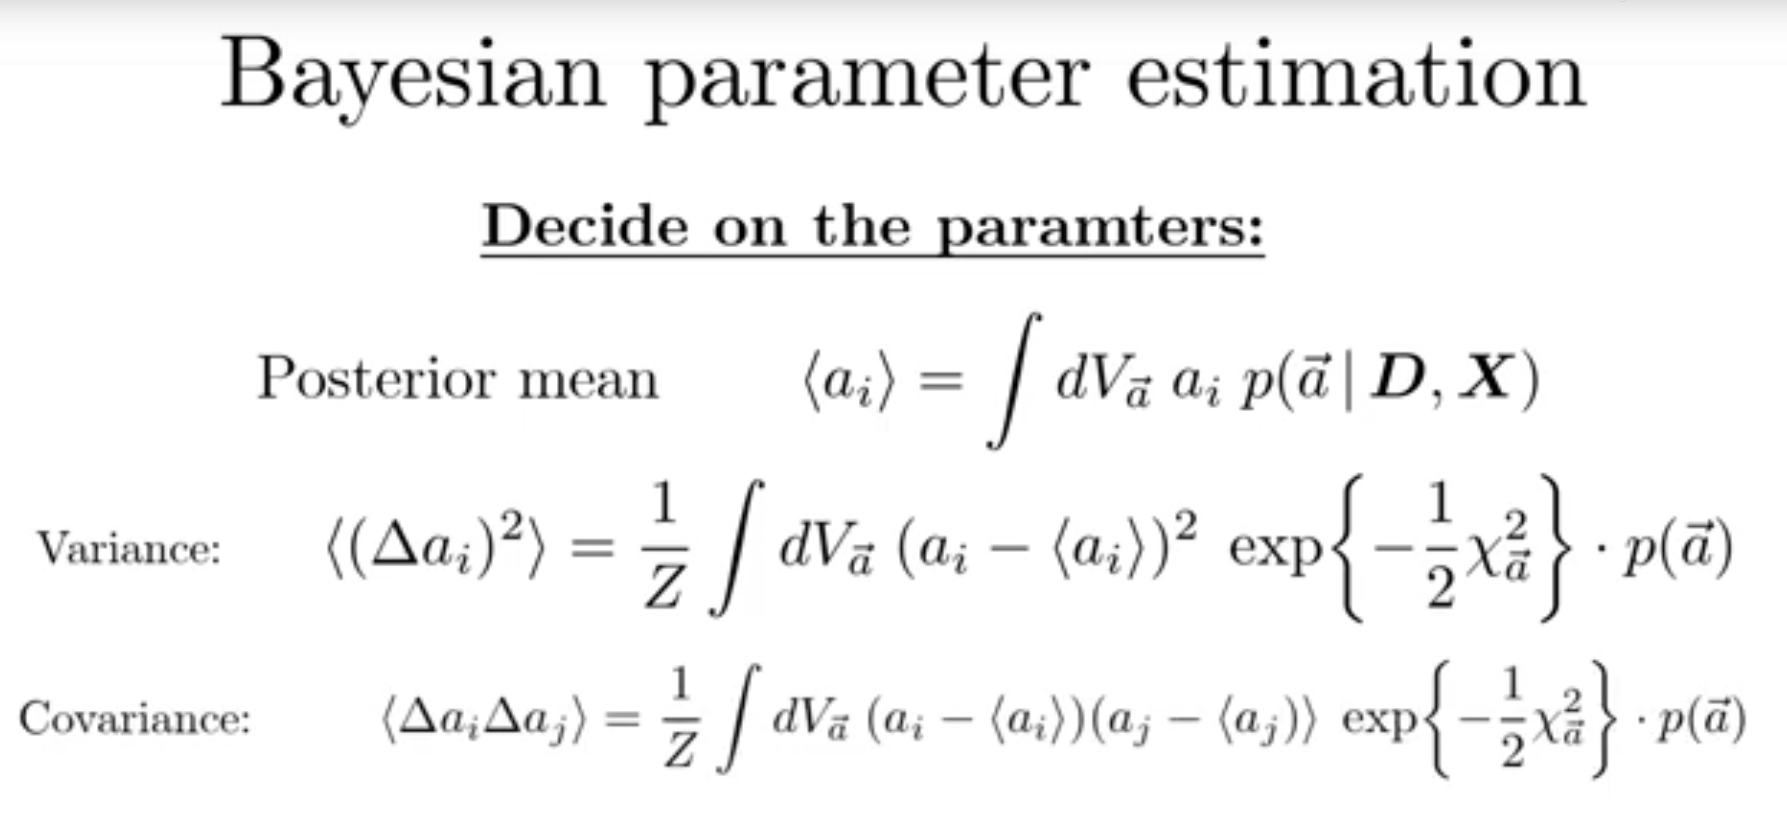
\includegraphics[width=0.75\textwidth]{7_7.png}
\end{figure}

It tells us whether uncertainties are correlated. For instance it could be that
only a combination $a_1 + a_2$ is well defined by the data, while the individual
values are not. This can be seen in the covariance.\\

\section*{Predicting values}
Now we turn to the predictive aspect of regression. We are interested in the
function value $y^*$ at a new position $x^*$, given the data $\boldsymbol{D}$. If the pivot point
$x^*$ lies \textit{within the set of given pivot points}, we call this type of prediction an
\textbf{interpolation}, otherwise \textbf{extrapolation}. The naive and inconsistent approach
would be to replace the unknown parameters by the estimated obtained before 
and just insert $x^*$ in the model function to obtain the function value
at the desired position. \\%7_8
\begin{figure}[H]
	\centering
	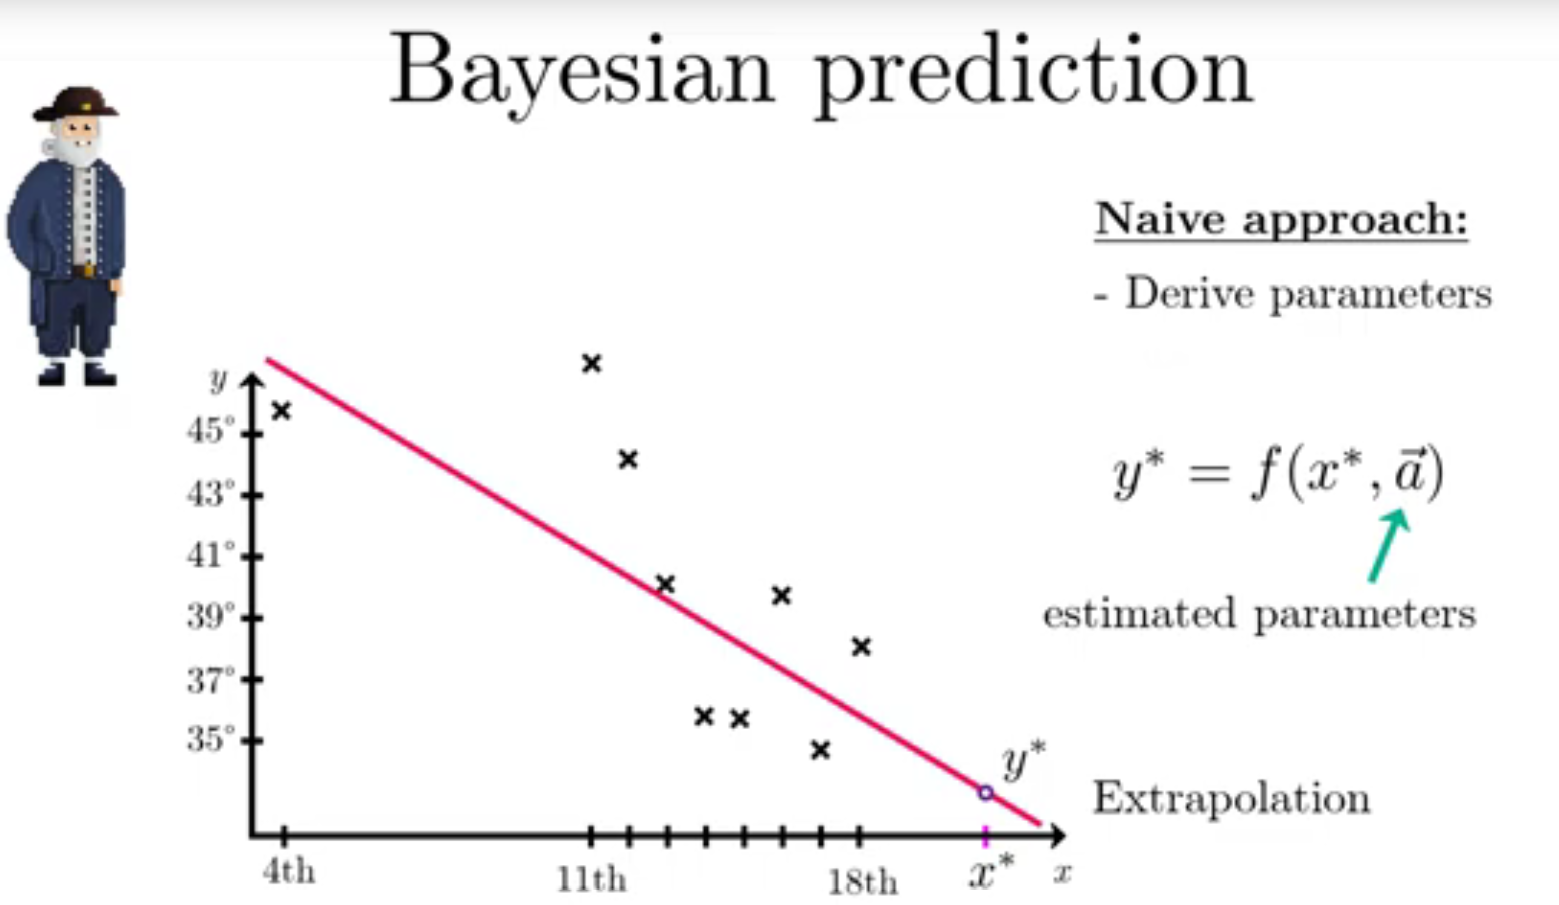
\includegraphics[width=0.75\textwidth]{7_8.png}
\end{figure}
The correct approach, however, is to \textit{determine the probability for the function 
value $y^*$ given the data, so $P(y^*|\boldsymbol{D},X)$}.
We can compute $p(y^*|\vec{a},\boldsymbol{D},X)=\delta(y^*-f(x^*,\vec{a}))$ if we know the parameters. So we introduce
them via the marginalization rule.%
\begin{equation*}\boxed{p(y^*|\boldsymbol{D},X)=\int \text{d}V_{\vec{a}}p(y^*|\vec{a},\boldsymbol{D},X) \cdot p(\vec{a}|\boldsymbol{D},X)
}\end{equation*}\\
 Then the moments of $y^*$ are 
 \begin{equation*}\boxed{\langle (y^*)^n\rangle=\int \text{d}V_{\vec{a}}(f(x^*,\vec{a}))^n \cdot p(\vec{a}|\boldsymbol{D},X)
}\end{equation*}\\
The result becomes particularly simple if the model function depends
linearly of the parameters, so $f(x,\vec{a})=M(x)\vec{a}$, where $M(x)$ is a row-vector containing the ansatz functions $M=(\Phi_1(x),\Phi_2(x),...)$
evaluated at $x$. Then the mean of the regression value $y^*$ is equal to the \textit{linear combination
of the ansatz functions with the mean of the parameters}.
\[\langle y^*\rangle = M(x^*)\langle \vec{a}\rangle\]
So in the linear case, this is in agreement with the naive approach, with the
parameters replaced by the posterior mean.
For the variance of the regression value we obtain
\[\langle (\Delta y^*)^2\rangle = M(x^*)CM^T(x^*)\]
The square root of the variance quantifies the uncertainty of the regression
value.\\%


Captain Venn wanted to know the azimutal or horizontal angles of the
star Arcturus at midnight on the shortest night of the year. Since the whether
was cloudy on that day of observation he wanted to infer the treasure's position
by interpolating his measurement values.\\
Captain Venn knows that the accuracy of his measurements is limited by
his time measurement which has an accuracy of about one minute. 
The uncertainty of his angle measurements is given by the \textit{sum of
the deviations due to the time shifts plus the accuracy of his sextant and compass}.
From test measurements he knows the approximate deviations of the angles due to the time inaccuracy.
We assume that the deviations of the angles are normal distributed with the derived $\sigma$ values just mentioned.%7_9
\begin{figure}[H]
	\centering
	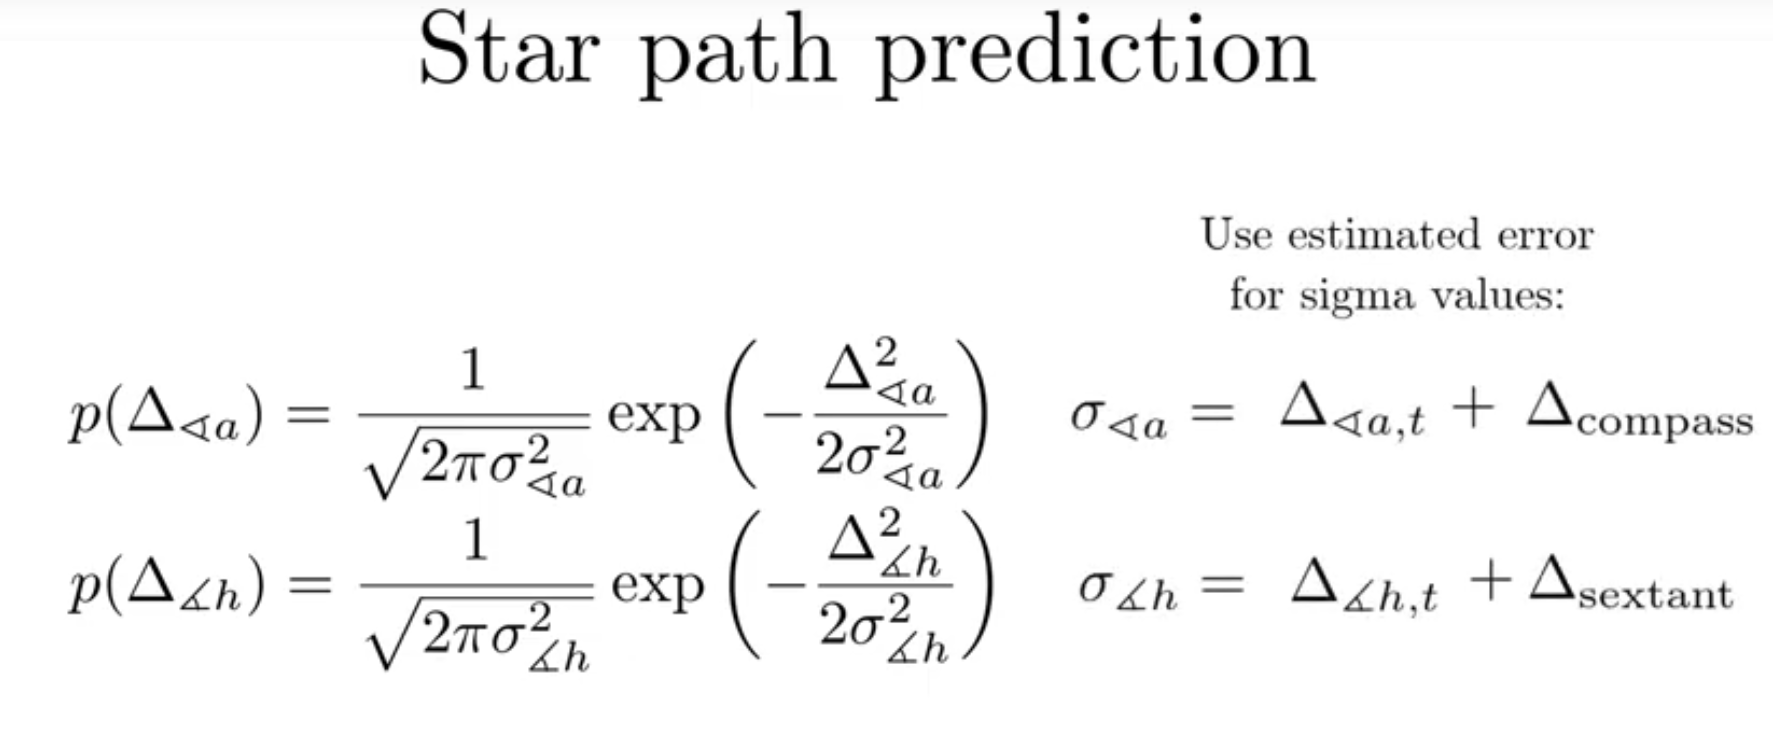
\includegraphics[width=0.75\textwidth]{7_9.png}
\end{figure}
Next we assume a linear model for which we can apply the formulas we just derived%7_10
\begin{figure}[H]
	\centering
	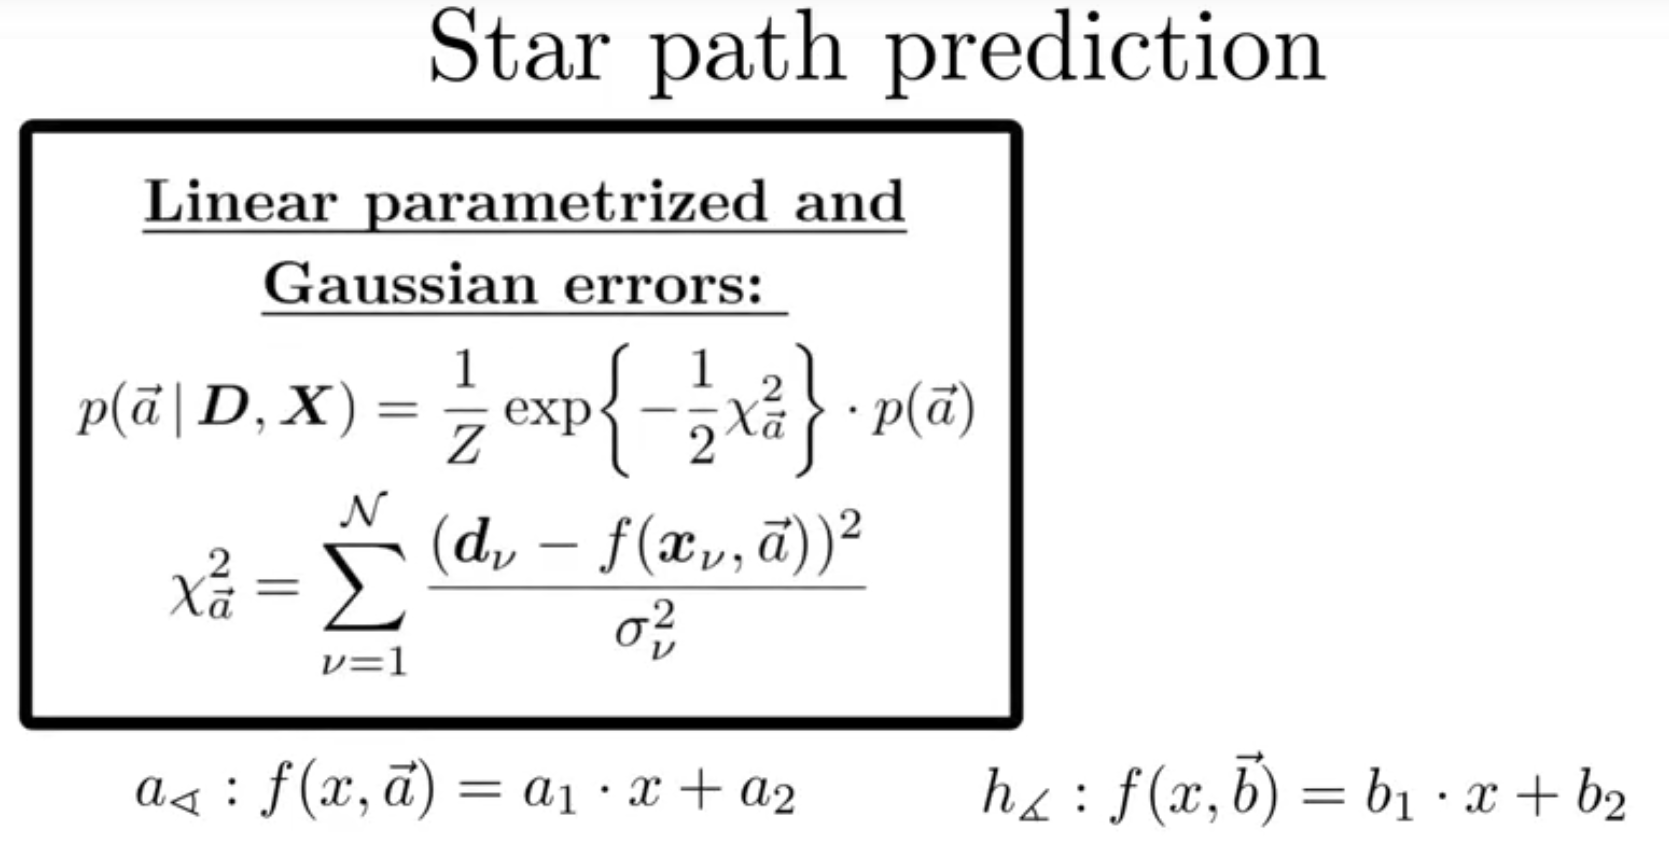
\includegraphics[width=0.75\textwidth]{7_10.png}
\end{figure}
formulas. Following the Bayesian regression steps we end up with a joint
probability density for the linear parameter and we can use them to derive a prediction for the desired angles.%7_11
\begin{figure}[H]
	\centering
	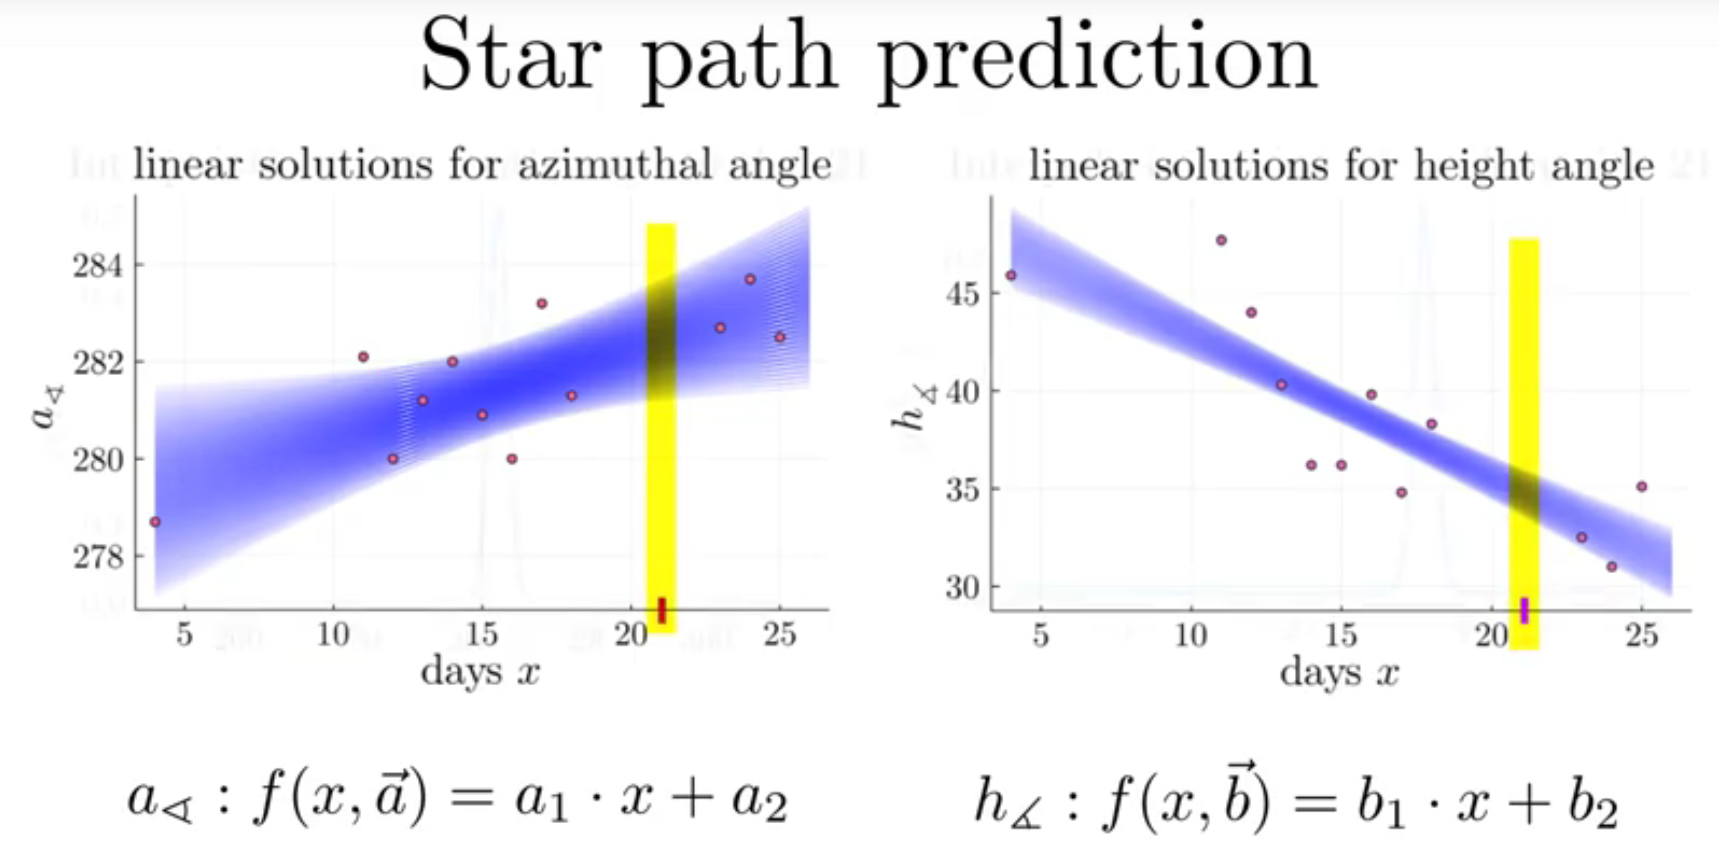
\includegraphics[width=0.75\textwidth]{7_11.png}
\end{figure}

\textit{Have a look at the interactive Pluto notebooks to get familiar with other
model functions and the numerical tricks to evaluate the integrals over the
whole parameter space! Here you can also explore the benefits of using a better 
astronomic model to predict star orbits and check how well extrapolation
works within several months.}\\

\section*{Classification}
Now we turn to the classification problem.
Given the \textit{classification labels} for the two species of fish and their \textit{positions}, the goal
is to \textit{find the border between the fish reserves}, which shall be described by
a linear function.\\%7_12
\begin{figure}[H]
	\centering
	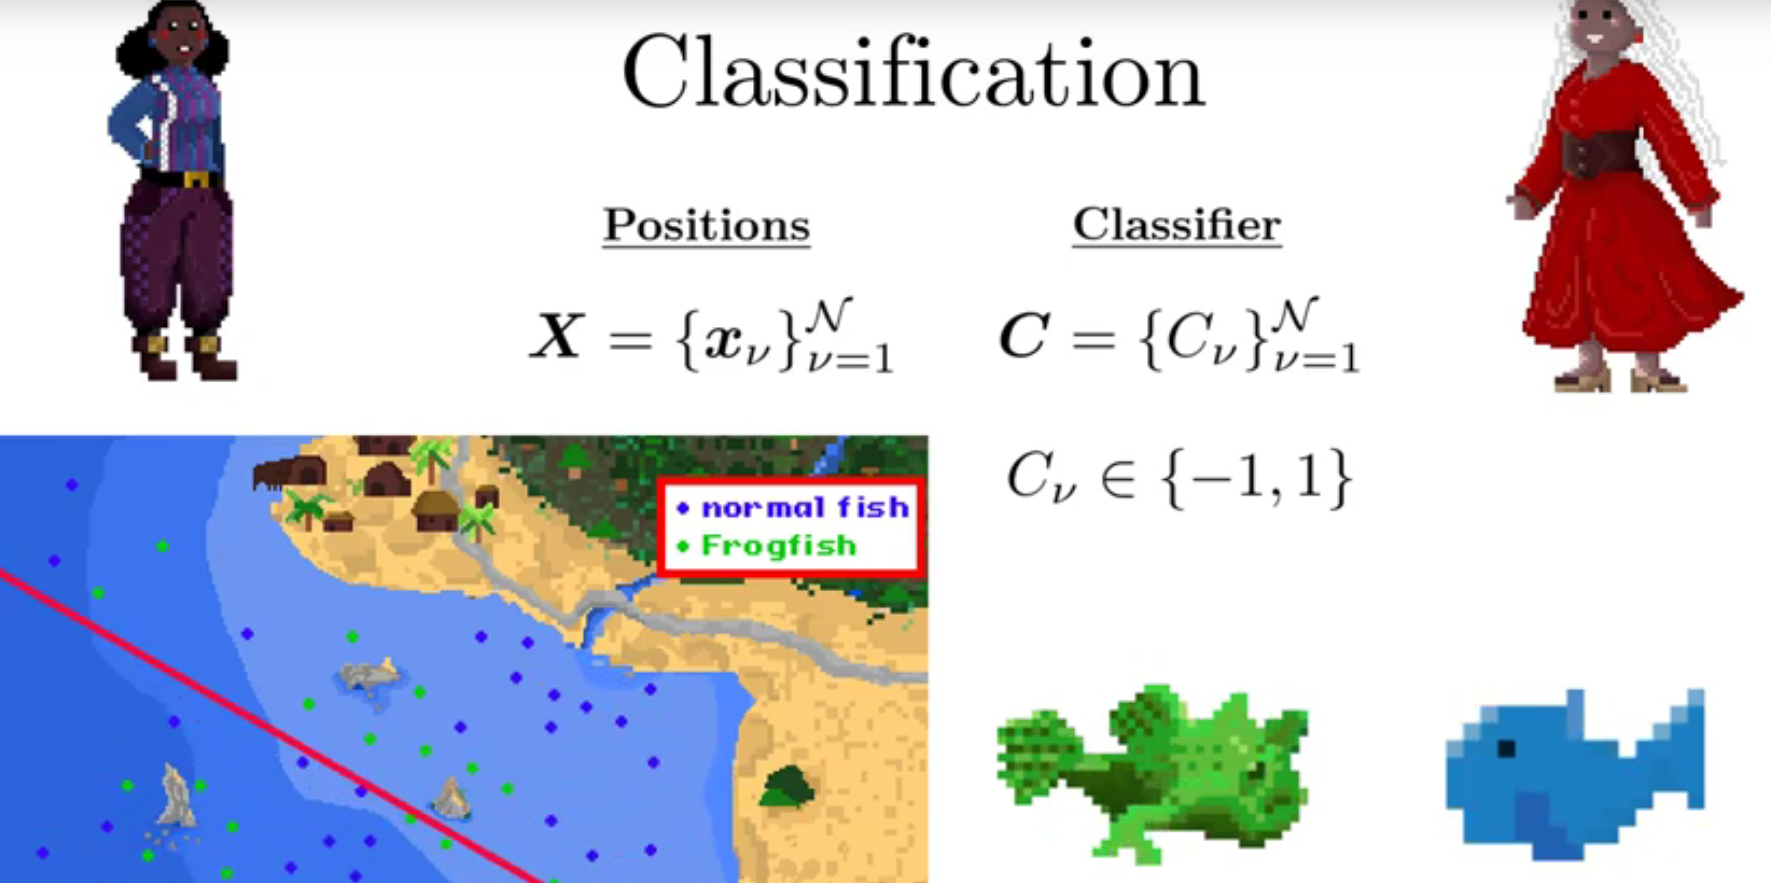
\includegraphics[width=0.75\textwidth]{7_12.png}
\end{figure}

The function depends on some parameters $\vec{a}$. 
\[y_{border}=f(x,\vec{a})=M(x)\vec{a}\]
Here $M_{ij}(x)=\phi_j(x_i)$ defines the model, or rather
the \textit{set of ansatz functions that are linearly combined weighted by the parameters}. For instance we can have a linear model or a quadratic model. We can also construct an implicit function. \[f(x,y,\vec{a})=M(x,y)\vec{a}=0\]
When we insert the position $(x_i|y_i)$ of the fish, the implicit function yields 0 if the fish resides exactly on the boundary. Otherwise the sign of the function tells us on which side of the boundary the fish is located. 
In order to derive the probability density for the model $p(\vec{a}|\boldsymbol{X},M,\boldsymbol{C})$
parameters given positions $\boldsymbol{X}$ and labels $\boldsymbol{C}$ of all fish and the model $M$, we proceed in a similar manner as in the regression case. Bayes’ theorem yields a proportionality to the product of likelihood and prior.\[p(\vec{a}|\boldsymbol{X},M,\boldsymbol{C})\propto p(\boldsymbol{X}|\vec{a},M,\boldsymbol{C})p(\vec{a}|M)\]

The classification label $\boldsymbol{C}$ has been omitted in the conditional part of the prior as it has no implications. 
Moreover we assume that the likelihood terms are \textit{uncorrelated} resulting in a product form. \[p(\boldsymbol{X}|\vec{a},M,\boldsymbol{C})=\prod_{\nu}p(\boldsymbol{x}_{\nu}|\vec{a},M,\boldsymbol{C}_{\nu}\]
The individual likelihood factors are the \textit{probability to find a fish of a certain species at a specific position}.
Here, the model and the corresponding parameters are important because they define the boundary of the fish reserves.
The likelihood is a \textit{property of the fish} and is related to why and how they stick to their reserve. 
The likelihood could in principle be quite different for the classification of other objects.
Nevertheless, the following considerations show how such classification problems are treated in
the framework of Bayesian probability theory in general.\\
As mentioned before, the sign of the implicit function $f(x_{\nu},y_{\nu},\vec{a})$ tells us on which side of the boundary the fish is located. \\

In the case of a linear implicit model function, the value of $f(x,y,\vec{a})=xa_1+ya_2+1$ can be used to easily determine the \textit{shortest distance to the boundary}. Just think of the Hessian normal form.%7_13
\begin{figure}[H]
	\centering
	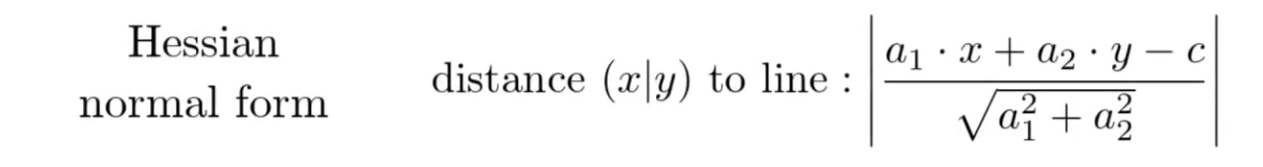
\includegraphics[width=0.75\textwidth]{7_13.png}
\end{figure}
%Generally for a fish at position $x_v$, we define the shortest distance to the border by the following expression.\\%

The distance is defined as positive if the fish is on the correct site of the boundary and negative otherwise.
In order to obtain a probability that is constant for a fish in its own reserve and that decreases continuously to zero when crossing the border we choose the logistic function.
The likelihood then reads%7_14
\begin{figure}[H]
	\centering
	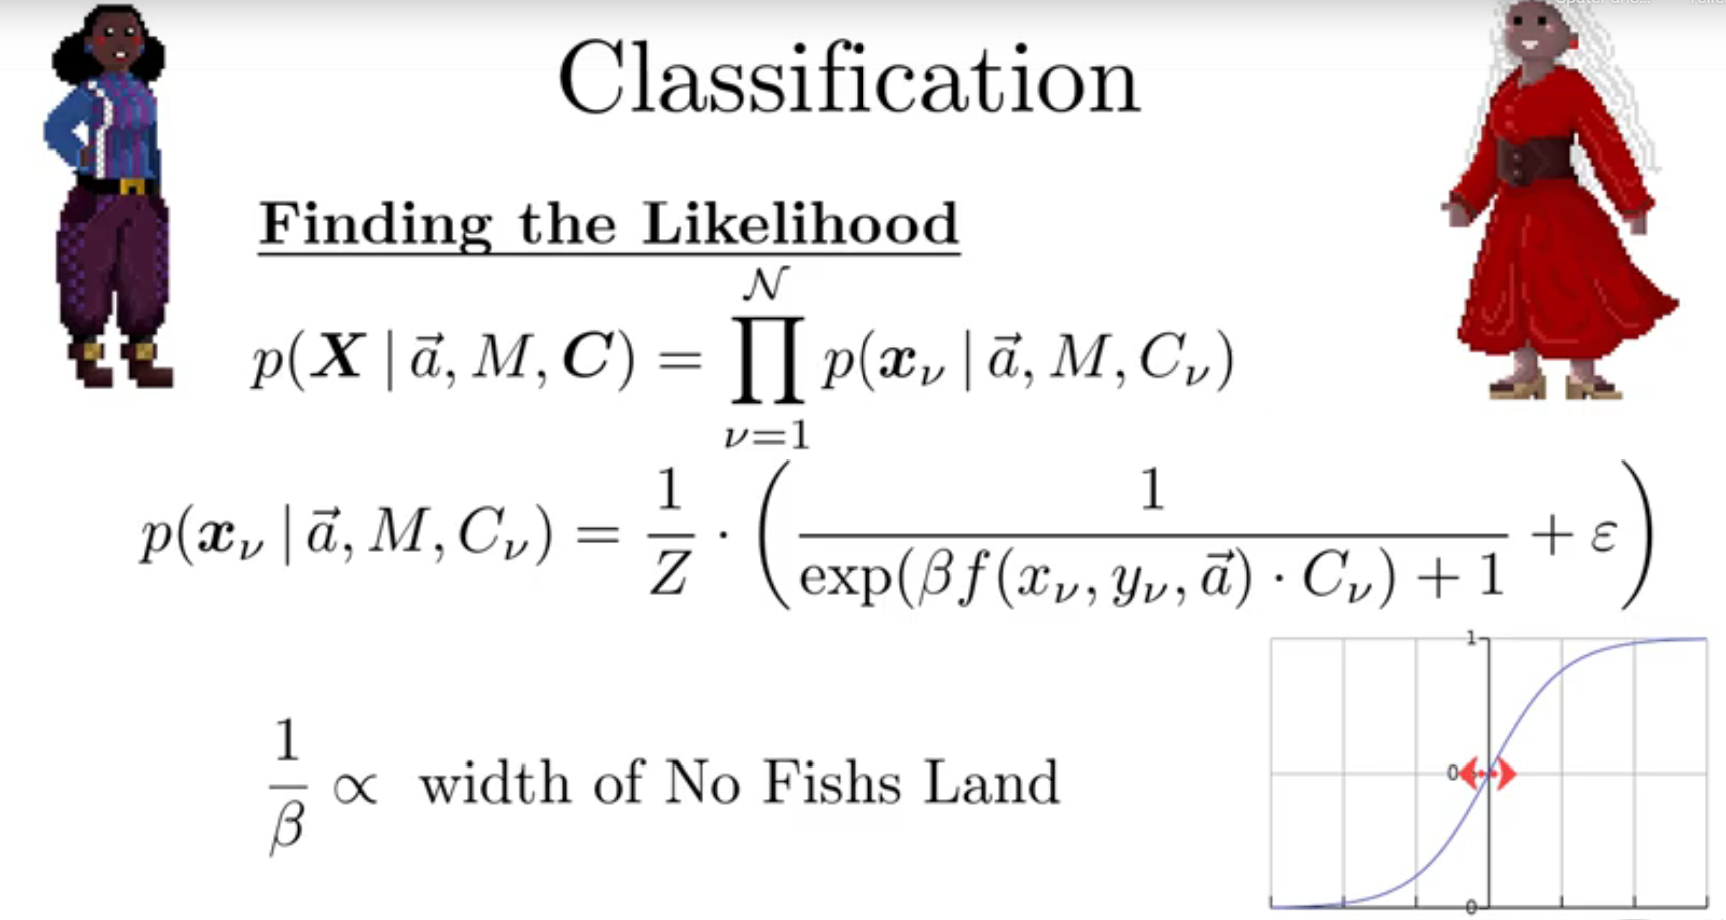
\includegraphics[width=0.75\textwidth]{7_14.png}
\end{figure}
where $\frac {1}{\beta}$ defines the width of the ``No Fish’s Land'' in which the probability
drops continuously to zero. 
Its area is assumed to be \textit{very small} and the logistic function is almost a step function. 
Hence the meaning of the \textbf{normalization} $Z$ is the \textit{size of the area of the two reserves}. For simplicity, we assume that the dependence of these areas on the parameters $\vec{a}$ and on the fish label $C_i$ can be ignored.
Then $Z$ is an unimportant constant.\\
It happens that not all fish abide by the rules. $\epsilon$ is the proportion of such fish and is related to the \textbf{slack variable}
in optimization problems. 
$\epsilon$ makes the classification \textbf{outlier tolerant}.
So by now we have all terms of the probability for the model parameters.
From that we can determine the mean values of the parameters, as well as their uncertainty. %7_15
\begin{figure}[H]
	\centering
	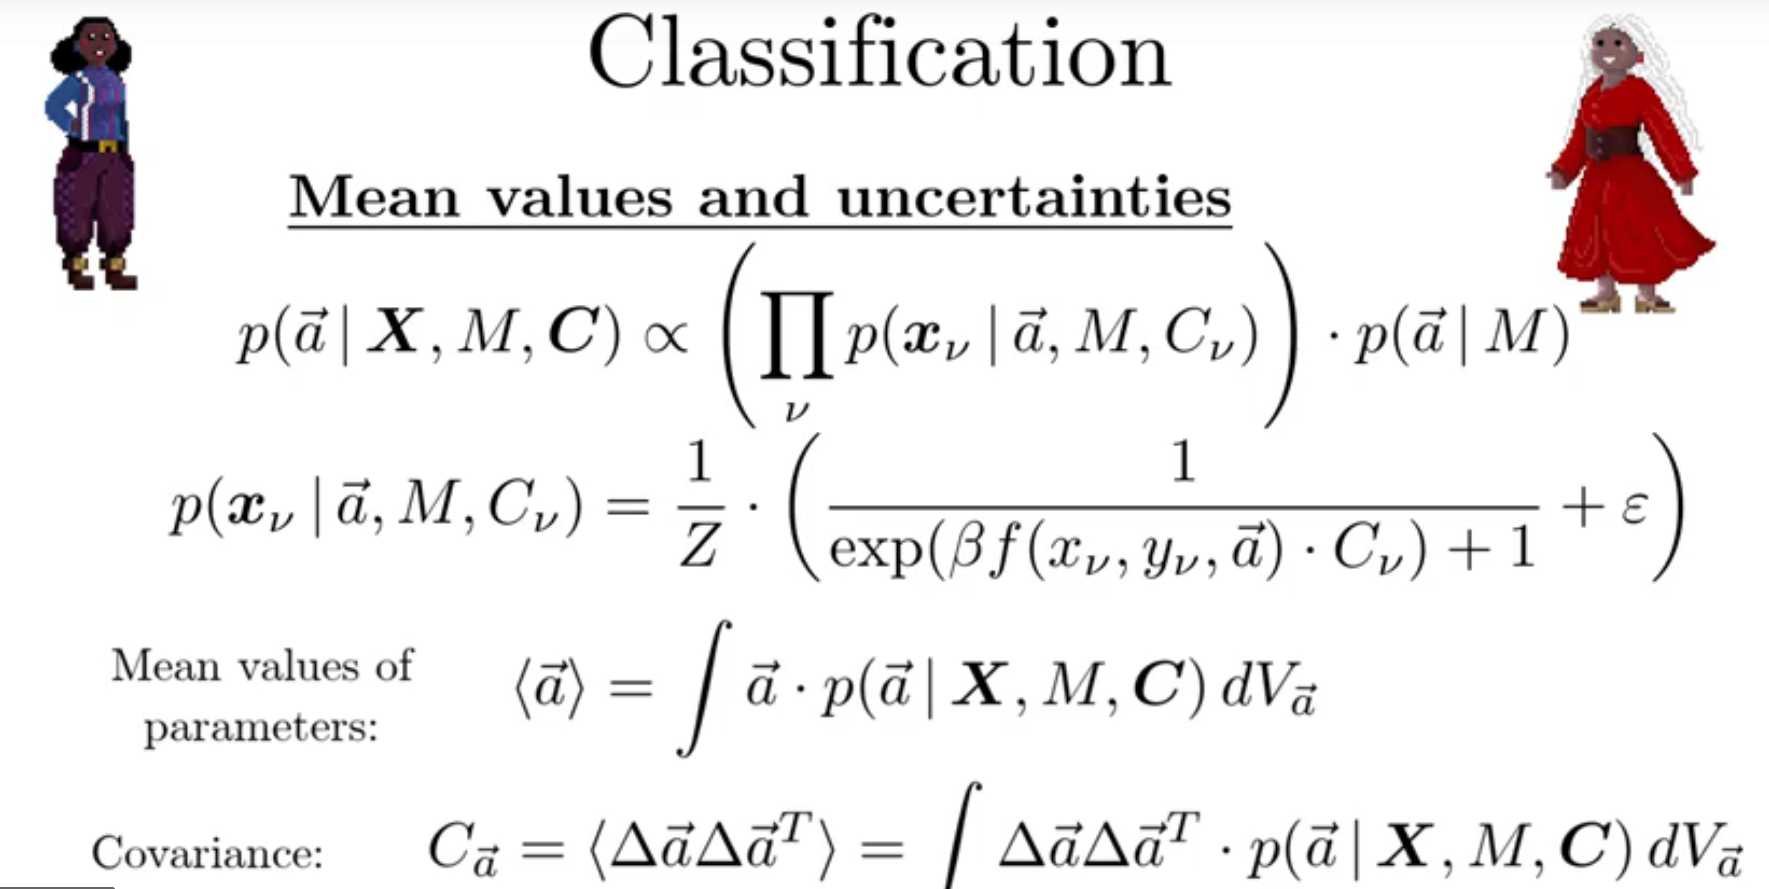
\includegraphics[width=0.75\textwidth]{7_15.png}
\end{figure}

Finally we can determine the mean and the variance of the boundary. 
\[\langle y\rangle =M(x)\langle \vec{a}\rangle \qquad C_y=\langle \Delta y \Delta y^T\rangle = M(x)C_{\vec{a}}M(x)^T\]

So let’s apply the Bayesian logistic classification approach to find the probability for the natural
boundary of the fish reserve. Using the data Bernoulli provided leads
to a probability distribution for the two parameters that can be visualized
by semitransparent borderlines.%7_16
\begin{figure}[H]
	\centering
	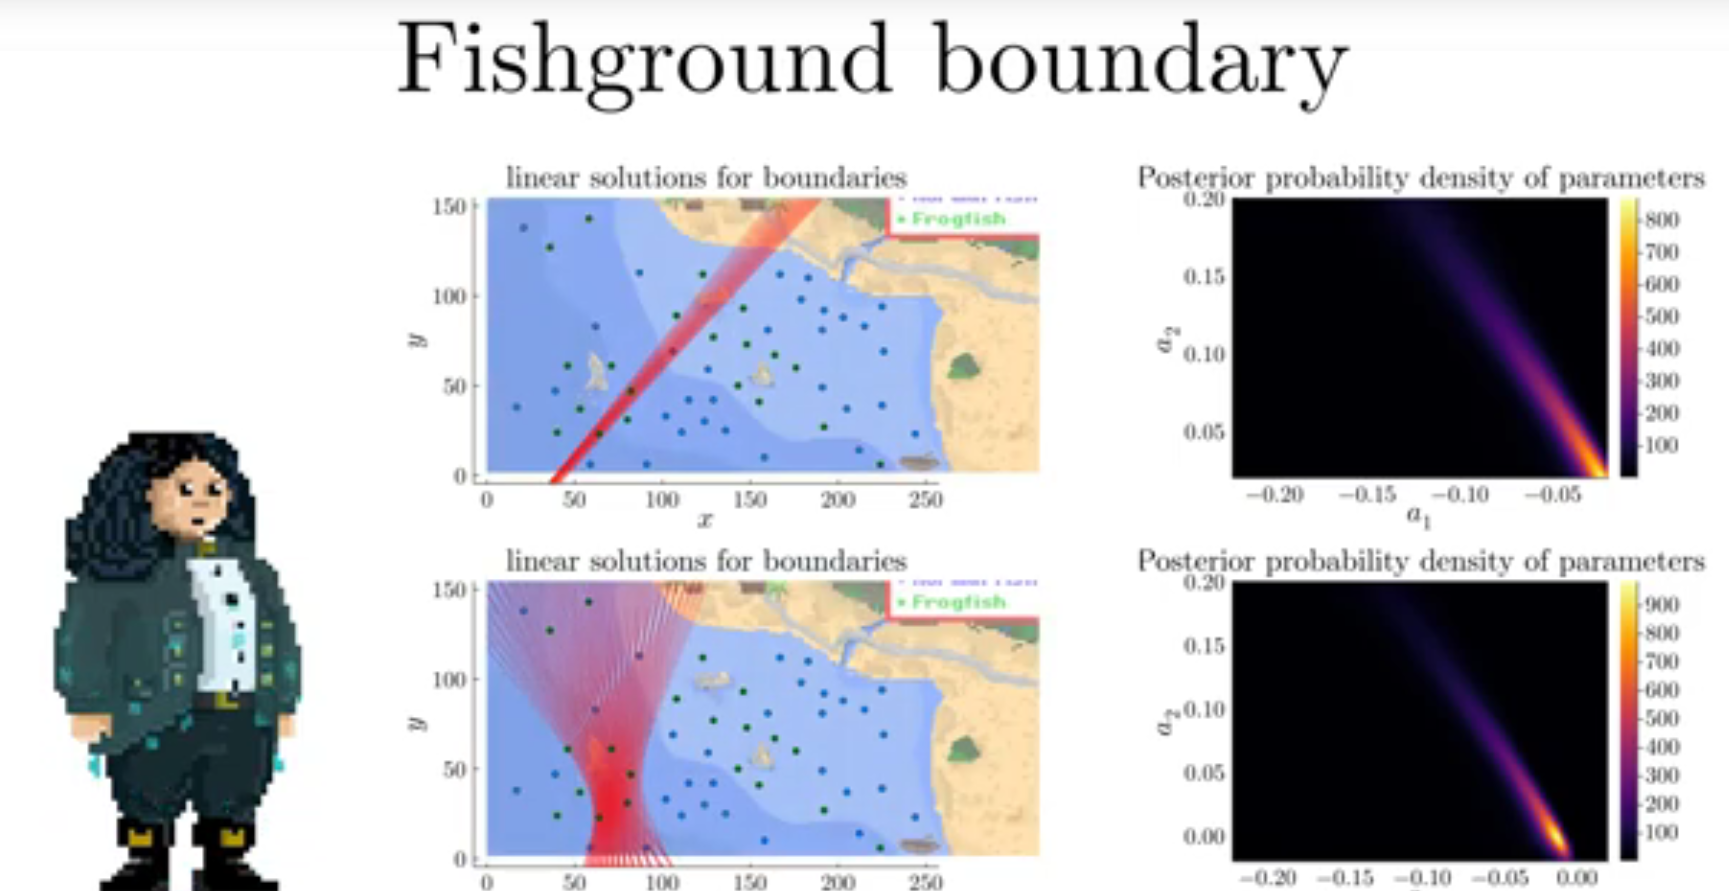
\includegraphics[width=0.75\textwidth]{7_16.png}
\end{figure}
 It can be seen from the formula that the likelihood function is maximized if the number of outliers is minimized. \\%7_17
 \begin{figure}[H]
 	\centering
	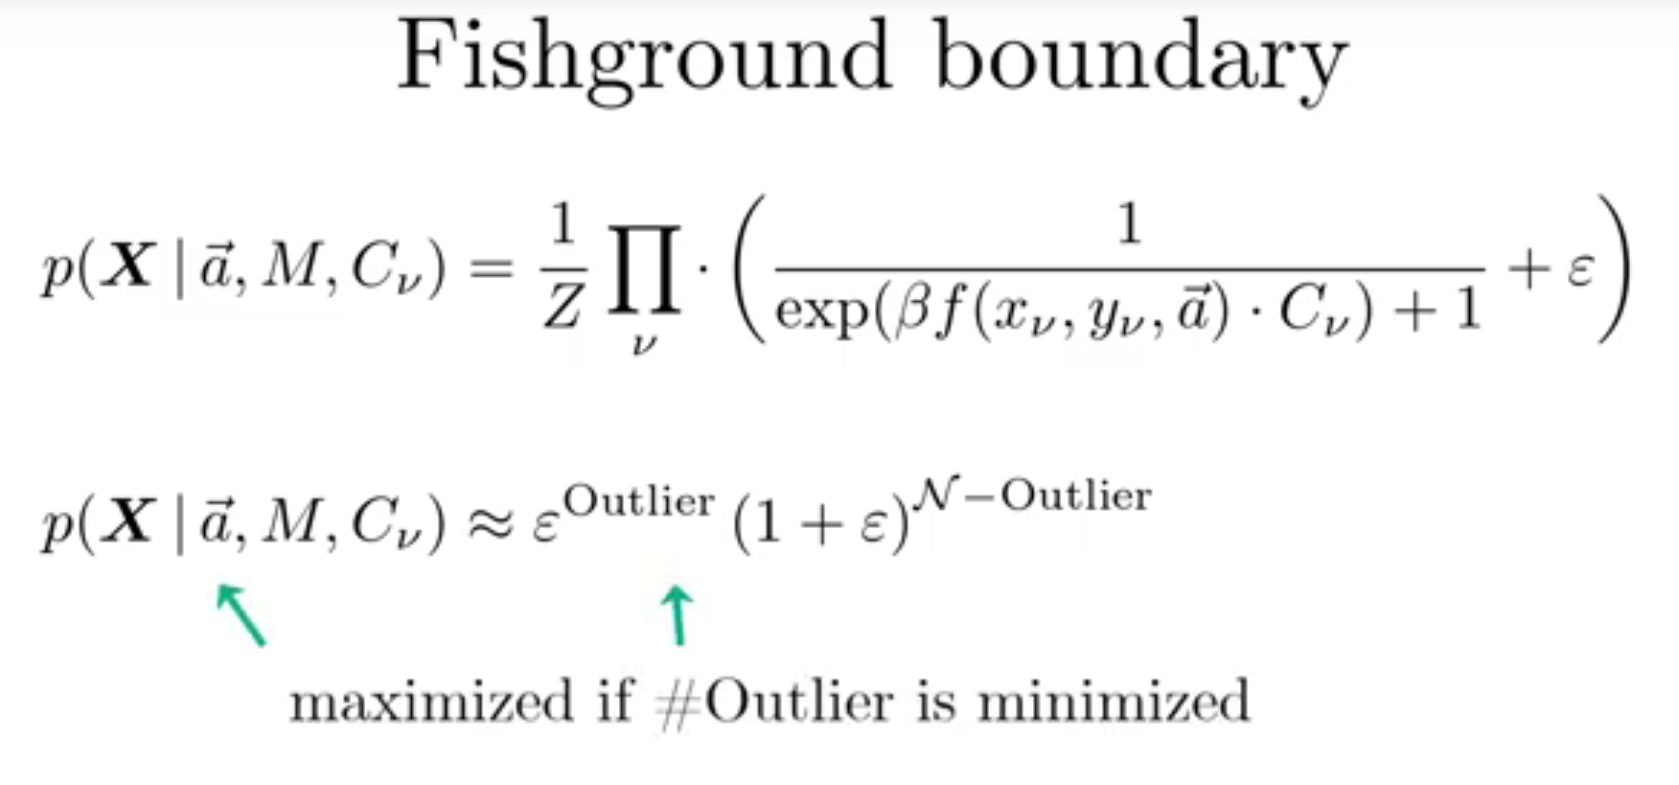
\includegraphics[width=0.75\textwidth]{7_17.png}
\end{figure}

\textit{See also the interactive pluto notebook to play with the slack variable $\epsilon$ and
other data sets.}\\

\section*{Model selection}
Another important question is the \textbf{model selection}, which answers the question ``\textit{What is the
probability that the correct form of the border is given by the model b, if we
know the position of all fish and their labels?}'' Here, Bayes theorem gives the following expression 
\[P(M|\boldsymbol{X},\boldsymbol{C})=\frac{1}{Z'}p(\boldsymbol{X}|M,\boldsymbol{C}) \cdot P(M,\boldsymbol{C})\]
where the normalization can easily be computed in the end.
Now we use the marginalization rule to introduce the model parameters.
As long as we do not know better, we assume a uniform prior within certain
parameter ranges.\\%7_18
\begin{figure}[H]
	\centering
	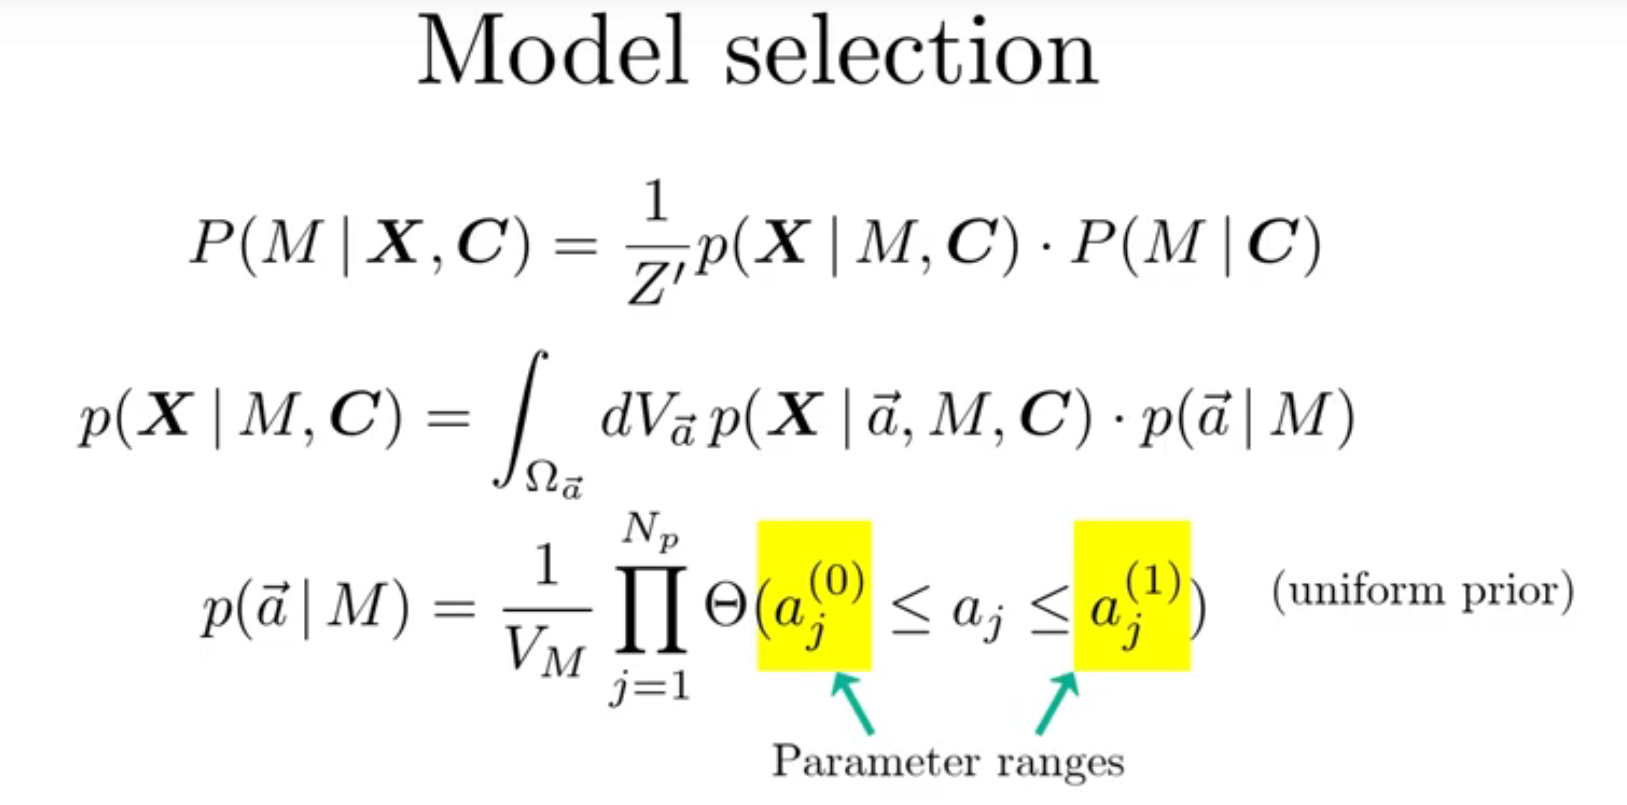
\includegraphics[width=0.75\textwidth]{7_18.png}
\end{figure}

Here $V_M$ is the prior volume that depends on the model.
Then the probability for model M in the light of the data is given by the following expression. %7_19
\begin{figure}[H]
	\centering
	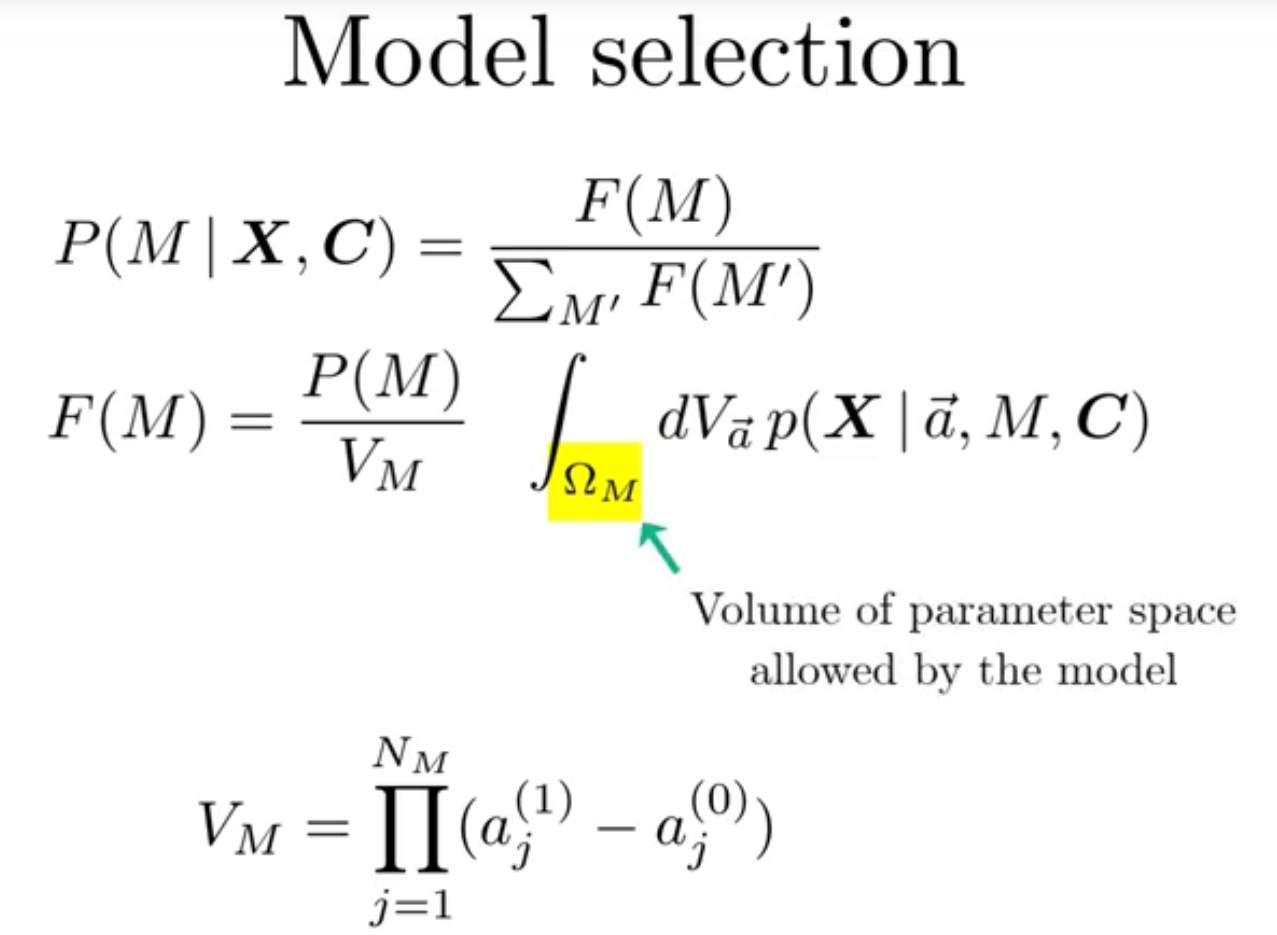
\includegraphics[width=0.75\textwidth]{7_19.png}
\end{figure}
Here $\Omega_M$ is the \textit{volume in parameter space} allowed by the model.
It should be noted that \textbf{Ockham's razor} is an integral part of the Bayesian expression 
and it \textit{penalizes unnecessarily complex models} \textit{(The more complicated a model is, the larger is its parameter volume!)}.\\
 

This concludes unit 7. We have learned Bayesian regression and how to
apply it to parameter estimation and model selection. 
We learned also how to predict unseen measurement values and their probabilities and we got insights into classification of data.
Now it’s your turn to actually find Captain Venn’s treasure in the pluto
notebooks where you can also work on the boundary issue of Claire and
Makabe.
Please feel free to ask questions in the forum and feel encouraged to test your
knowledge in the quiz!


\vspace{2cm}
\begin{minipage}[t]{1\textwidth}
	\raggedleft
	\centering
	
\includegraphics[width = 0.20\textwidth]{CC-BY_icon}
	\vspace{0.2cm}
	
	\centering
	{\large ITPCP, TU Graz} \\
	https://creativecommons.org/licenses/by/4.0/legalcode
\end{minipage}
\end{document}